\documentclass[a4paper]{article}

\usepackage[T1]{fontenc}	
\usepackage{amsmath}
\usepackage{amssymb}
\usepackage{fancyhdr}
\usepackage{booktabs}
\usepackage{graphicx}
\usepackage{float}

\pagestyle{fancy}
\rhead{Home Assignment 1}
\lhead{Noah Hansson \& Kristoffer Nordström}

\title{Home Assignment 1 - FMSN50}
\author{Kristoffer Nordström, Noah Hansson}\author{Kristoffer Nordström \\ kr8245no-s@student.lu.se \and  Noah Hansson \\ no3822ha-s@student.lu.se}
\date{\today}


\setlength{\parskip}{0.7em}
\setlength{\parindent}{0pt}
\setlength{\floatsep}{6pt plus 1.0pt minus 2.0pt}
\setlength{\textfloatsep}{10pt plus 1.0pt minus 2.0pt}

\begin{document}
\maketitle
\newpage

 
\section{Random Number Generation}\label{sec:RNG}
\subsection*{a)}
We are interested in finding the conditional distribution function of a stochastic variable $X$ given that $X$ is within a given interval, i.e $F_{X|X\in I}(x)$, where $I$ is the closed interval $I = [a,b]$. Using the law of total probability we can express this as:
\begin{equation}
    F_{X|X\in{I}}(x) = \frac{\int_a^xf_X(x)dx}{c} = \frac{\int_a^xf_X(x)dx}{\int_a^bf_X(x)dx} = \frac{F_X(x)-F_X(a)}{F_X(b)-F_X(a)}
    \label{acdf}
\end{equation}
Where $c$ is a normalising constant. From this we can easily compute the conditional probability density function:
\begin{equation}
    f_{X|X\in{I}}(x) = \frac{dF_{X|X\in{I}}(x)}{dx} = \frac{f_X(x)}{F_X(b)-F_X(a)}
\end{equation}

\subsection*{b)}
By the definition of an inverse distribution we want to find a probability distribution function $F_{X|X \in I}^{-1}(u)$ such as:
\begin{equation}
    F_{X|X \in I}(F_{X|X \in I}^{-1}(u)) = u
    \label{inverse}
\end{equation}
where $u$ is a variable sampled from a uniform distribution $u \sim U[0,1]$. Rewriting the left side in (\ref{inverse}) with (\ref{acdf}) gives us the following expression:
\begin{equation}
    \frac{F_X(F_{X|X\in I}^{-1}(u))-F_X(a)}{F_X(b)-F_X(a)} = u
\end{equation}
Solving for $F_{X|X\in I}^{-1}(x)$ gives us:
\begin{equation}
    F_{X|X\in I}^{-1}(u) = F_X^{-1}((F_X(b)-F_X(a))u + F_X(a))
    \label{finvers}
\end{equation}

By using this it's possible to simulate samples from a uniform distribution and then calculate the inverse in (\ref{finvers}) to get a conditionally simulation of $X \in I$.

\newpage
\section{Power Production of a Wind Turbine}
\label{sec:oneTurbine}

\subsection*{a) Crude Monte-Carlo sampling}
To calculate an initial estimate of the power production of the Wind Turbine we start by sampling the power production using regular Monte-Carlo sampling. We begin by generating $10^5$ samples of wind distributed by a Weibull distribution for each month. We then calculate the generated power for each wind sample and then find the average and the variance for each month. The estimate is calculated as follows:
\begin{equation}
    \tau = \mathbb{E}[\phi(X)] = \frac{1}{N}\sum_{i = 1}^N\phi(X_i)
\end{equation}
And since the sample size is large we can also assume that the central limit theorem applies, giving us:
\begin{equation}
    \mathbb{V}[\sqrt{N}(\tau_N-\tau)] = N\mathbb{V}[\tau_N-\tau] = \mathbb{V}[\phi(X)]
\end{equation}
In this case the stochastic variable $X$ is the wind speed and $\phi(X)$ is the power curve function for the wind turbine.

The results are presented in table \ref{tab:CrudeResults} and the samples for january are plotted in figure \ref{fig:samplesJan}.
\begin{table}[H]
    \centering
    \caption{Crude Monte Carlo estimates and confidence intervals of power production for each month of the year}
    \label{tab:CrudeResults}
    \begin{tabular}{lllr}
\toprule
{} &   Mean [kW] &        Interval &     Variance  \\
Month &             &                 &               \\
\midrule
jan   &  1729398.04 &   $\pm$ 7586.68 &  1.498275e+12 \\
feb   &  1574090.66 &   $\pm$ 7528.13 &  1.475237e+12 \\
mar   &  1466612.49 &   $\pm$ 7426.44 &  1.435653e+12 \\
apr   &  1190918.98 &   $\pm$ 7107.77 &  1.315086e+12 \\
may   &  1139016.09 &   $\pm$ 6969.14 &  1.264290e+12 \\
jun   &  1210539.74 &   $\pm$ 7135.69 &  1.325438e+12 \\
jul   &  1143510.67 &   $\pm$ 7000.18 &  1.275577e+12 \\
aug   &  1213284.01 &   $\pm$ 7149.09 &  1.330423e+12 \\
sep   &  1444936.39 &   $\pm$ 7415.53 &  1.431438e+12 \\
oct   &  1586902.48 &   $\pm$ 7629.18 &  1.515106e+12 \\
nov   &  1731424.95 &   $\pm$ 7584.78 &  1.497524e+12 \\
dec   &  1722549.05 &   $\pm$ 7586.04 &  1.498021e+12 \\
\bottomrule
\end{tabular}

\end{table}

\begin{figure}[H]
    \centering
    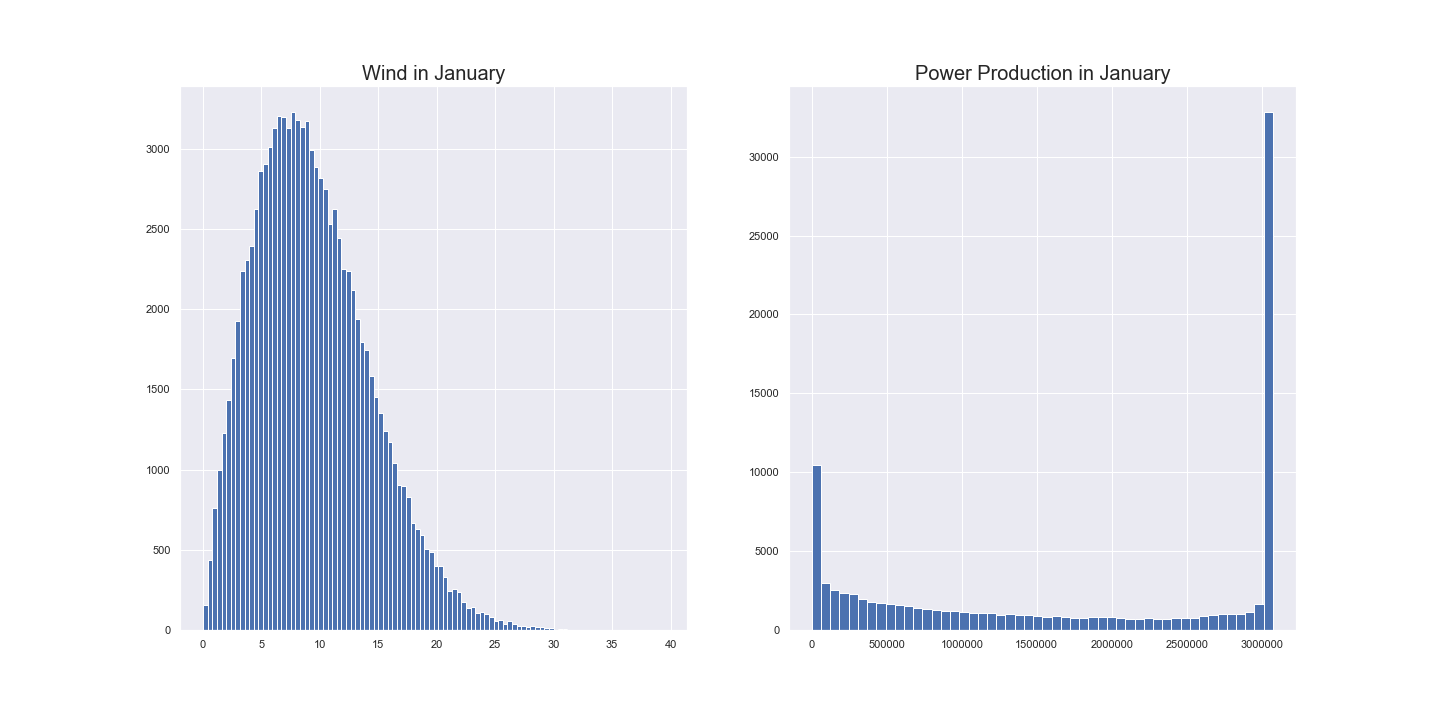
\includegraphics[width = 1.0\textwidth]{images/janCrudeMC}
    \caption{Sampled wind speed (left) and power production (right) for January}
    \label{fig:samplesJan}
\end{figure}

Since we know that the wind turbine produces no power when the wind speed is above 25 m/s or below 3 m/s we can modify our Monte Carlo simulation by truncating our wind samples. Using the results in section \ref{sec:RNG} we can instead generate wind samples within the interval $[3,25]$ m/s to reduce the variance of $\tau$. In order to compensate for the truncation we then multiply the estimates by the probability that the wind speed is within the interval.

The results are presented in table \ref{tab:CrudeResultsTrunc} and the samples for january are plotted in figure \ref{fig:samplesJanTrunc}.
\begin{table}[H]
    \centering
    \caption{Crude Monte Carlo estimates and confidence intervals of power production for each month of the year using truncated wind samples}
    \label{tab:CrudeResultsTrunc}
    \begin{tabular}{lllr}
\toprule
{} & $\tau$ [kW] &      $I_{95\%}$ &  $\mathbb{V}(\tau)$ \\
Month &             &                 &                     \\
\midrule
jan   &  1731719.18 &   $\pm$ 6597.59 &        1.133075e+12 \\
feb   &  1566574.66 &   $\pm$ 6533.15 &        1.111049e+12 \\
mar   &  1466464.51 &   $\pm$ 6426.78 &        1.075165e+12 \\
apr   &  1192070.88 &   $\pm$ 5940.35 &        9.185679e+11 \\
may   &  1135596.02 &   $\pm$ 5830.83 &        8.850116e+11 \\
jun   &  1211715.53 &    $\pm$ 5994.8 &        9.354866e+11 \\
jul   &  1147073.32 &   $\pm$ 5838.47 &        8.873321e+11 \\
aug   &  1211018.41 &   $\pm$ 5992.59 &        9.347962e+11 \\
sep   &  1446737.76 &   $\pm$ 6390.57 &        1.063082e+12 \\
oct   &  1585950.52 &    $\pm$ 6531.4 &        1.110452e+12 \\
nov   &  1731702.22 &   $\pm$ 6609.87 &        1.137295e+12 \\
dec   &  1726024.48 &   $\pm$ 6602.99 &        1.134929e+12 \\
\bottomrule
\end{tabular}

\end{table}

\begin{figure}[H]
    \centering
    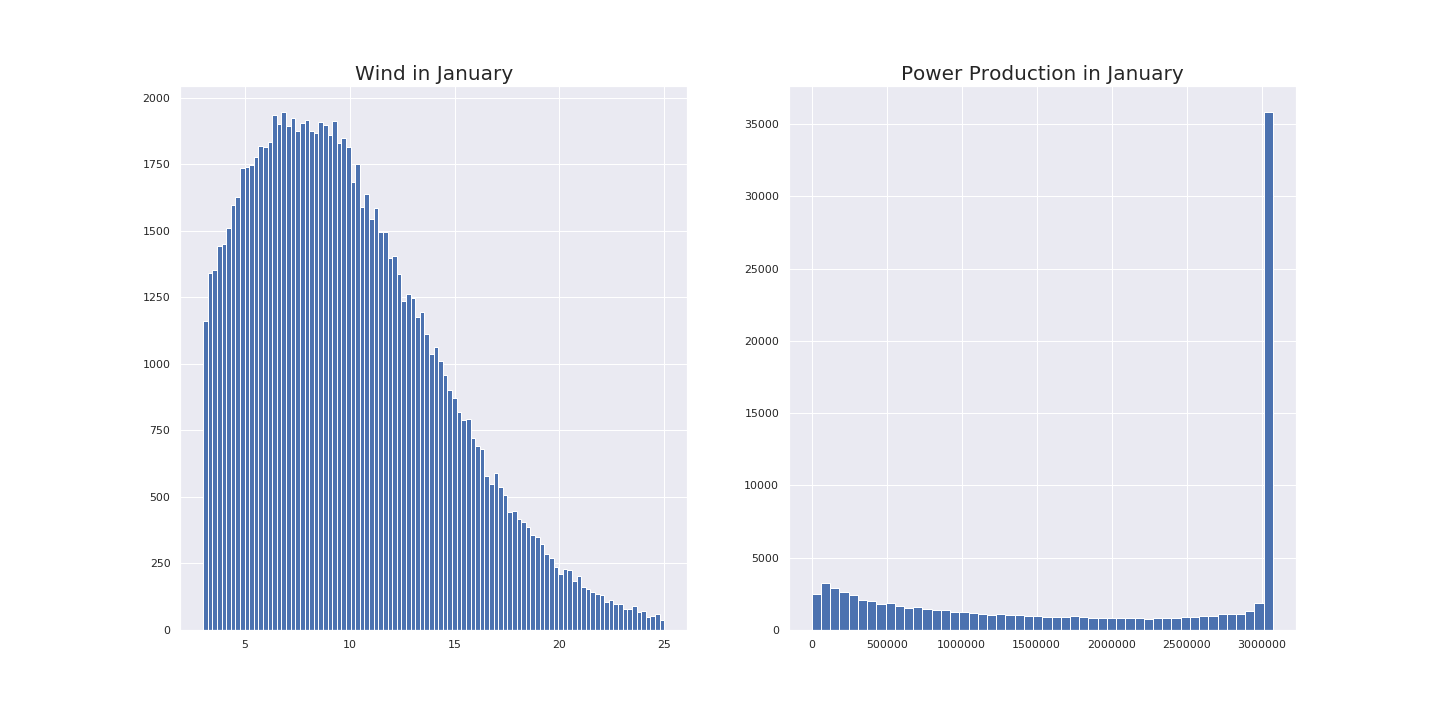
\includegraphics[width = 1.0\textwidth]{images/janCrudeMCTrunc}
    \caption{Sampled truncated wind speed (left) and power production (right) for January}
    \label{fig:samplesJanTrunc}
\end{figure}


\subsection*{b) Importance Sampling}
To reduce the variance of the Monte-Carlo estimate we will here apply the importance sampling method. When we generate random wind samples we sometimes get samples of wind speed that give us a power production of zero. These samples give do not help finding a better estimate of the average power, as they only increase the variance of the estimator. Instead, we try to find an instrumental density g where we then draw our wind samples from. This reduces the amount of "bad" samples and reduces the variance of the estimator. \noindent To find an estimate of the average power production we use the following calculations, where the density $g(x)$ is a density such as $g(x) = 0 \rightarrow \phi(x)f(x) = 0$
\begin{equation}
    \begin{gathered}
        \tau = \mathbb{E}_f(\phi(X)) = \int_{|\phi(x)|f(x)>0}\phi(x)f(x)dx = \int_{g(x)>0}\phi(x)\frac{f(x)}{g(x)}g(x)dx = \\
        = \mathbb{E}_g[\phi(x)\frac{f(x)}{g(x)}] = \mathbb{E}_g[\phi(X)\omega(X)]
    \end{gathered}
\end{equation}
where
\begin{equation}
    \omega : \{x \in X : g(x)>0 \} \ni x \rightarrow \frac{f(x)}{g(x)}
\end{equation}
This gives us the estimates of $\tau$ as
\begin{equation}
    \tau = \mathbb{E}_g[\phi(X)\omega(X)]
\end{equation}
with the variance
\begin{equation}
    \mathbb{V}[\tau_N] = \frac{1}{N}\mathbb{V}_g[\phi(X)\omega(X)]
\end{equation}

In practice, we aim at finding a distribution $g(x)$ that resembles $f(x)\phi(x)$ and has a support that includes the whole support of $f(x)\phi(x)$. We then fine tune $g(x)$ such that the function $\phi(x)\omega(x)$ is close to constant in the support of $g(x)$. We then draw $10^5$ samples from $g(x)$ as the stochastic variable $X$ to estimate $\tau$. The results are presented in table \ref{tab:ISresults}. In this case we choose $g(x)$ as a normal distribution.

\begin{table}[H]
    \centering
    \caption{Importance Sampling Monte Carlo estimates and confidence intervals of power production for each month of the year}
    \label{tab:ISresults}
    \begin{tabular}{lll}
\toprule
Month & $\tau$ [kW] &   $I_{95\%}$ \\
\midrule
  Jan &     1730.18 &   $\pm$ 3.02 \\
  Feb &     1570.83 &   $\pm$ 2.68 \\
  Mar &     1468.02 &   $\pm$ 2.56 \\
  Apr &     1187.48 &    $\pm$ 2.5 \\
  May &     1138.65 &   $\pm$ 2.43 \\
  Jun &     1211.77 &   $\pm$ 2.54 \\
  Jul &     1141.39 &   $\pm$ 2.42 \\
  Aug &     1211.93 &   $\pm$ 2.53 \\
  Sep &     1447.62 &   $\pm$ 2.55 \\
  Oct &     1587.56 &   $\pm$ 2.75 \\
  Nov &     1730.17 &   $\pm$ 3.04 \\
  Dec &     1731.64 &   $\pm$ 3.02 \\
\bottomrule
\end{tabular}

\end{table}

\begin{figure}[H]
    \centering
    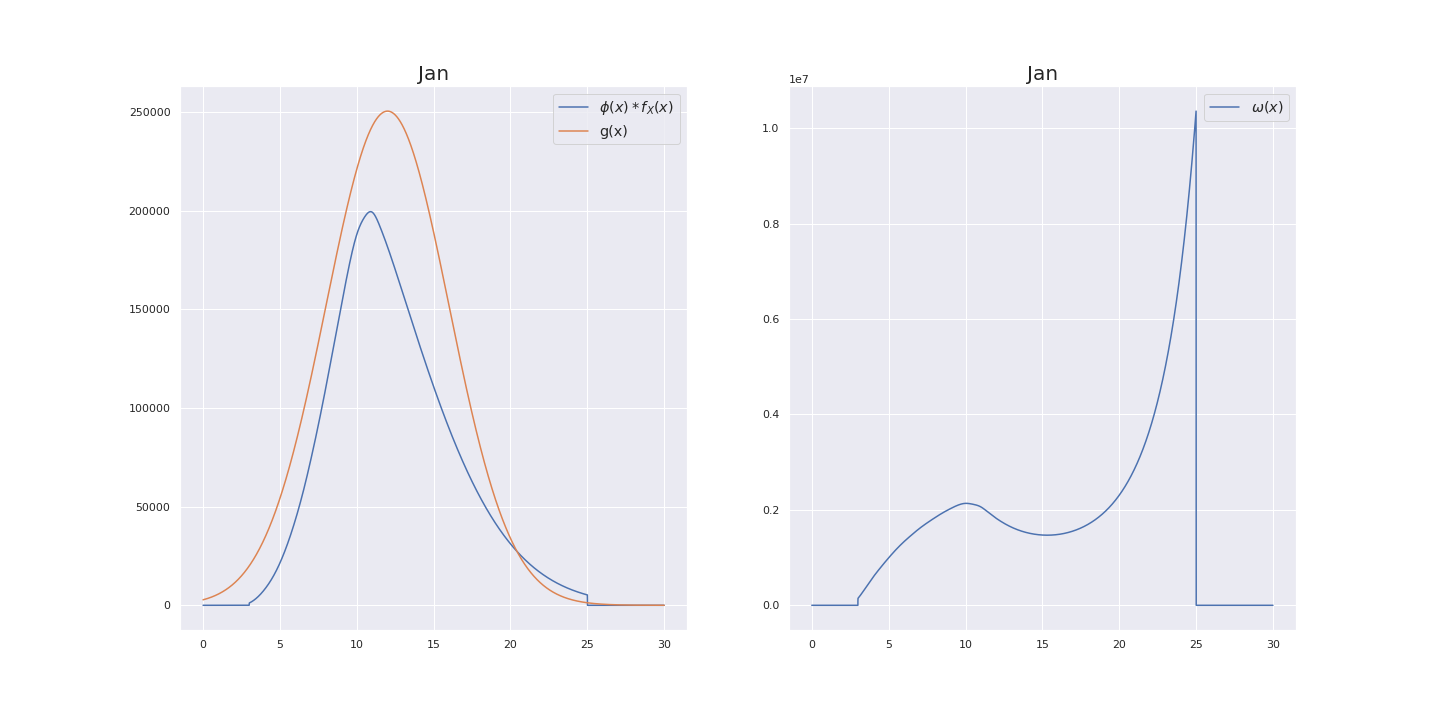
\includegraphics[width = 1.0\textwidth]{images/janISMC}
    \caption{$g(x)$ (scale-transformed) and $\phi(x)*f_X(x)$ (left) and $\omega(x)$ (right) for January}
    \label{fig:ISMCjan}
\end{figure}

\subsection*{c) Antithetic sampling}
Another method of reducing the variance is to use antithetic sampling to estimate $\tau = \mathbb{E}_f[\phi (X)]$ by defining the variable $V \overset{\mathrm{def}}{=} \phi (X)$ so that $\tau = \mathbb{E}[V]$. Then we find another variable $V^\prime$ with the same mean and distribution as $V$, but with a negative covariance. Then, if we define $$W \overset{\mathrm{def}}{=} \frac{V + V^\prime}{2}$$ it holds that $\mathbb{E}[W] = \tau$ and $$\mathbb{V}[W] = \frac{1}{2}(\mathbb{V}[V] + \mathbb{C}[V, V^\prime])$$Since the covariance between $V$ and $V^\prime$ is negative we should be able to find an estimate of $\tau$ with a lower variance than when using crude Monte Carlo.

In this case, we find $V$ and $V^\prime$ by evaluating the power fuction $P(V)$ of sampled wind using the inverse conditional weibull distribution. This gives us
\begin{equation}
    V = P(F_{X|X\in I}^{-1}(u))
\end{equation}
and
\begin{equation}
    V^\prime = P(F_{X|X\in I}^{-1}(1-u))
\end{equation}

Generating $10^5$ samples of $u$ and running each sample through both inverse distributions before evaluating the power production from those samples gives us the two stochastic variables $V$ and $V^\prime$ This gives us two identically distributed wind samples with negative covariance. The results are presented in table \ref{tab:ATresults}.

\begin{table}[H]
    \centering
    \caption{Antithetic Monte Carlo estimates and confidence intervals of power production for each month of the year}
    \label{tab:ATresults}
    \begin{tabular}{lll}
\toprule
Month & $\tau$ [kW] &  $I_{95\%}$ \\
\midrule
  Jan &     1730.89 &  $\pm$ 1.22 \\
  Feb &     1570.29 &  $\pm$ 0.53 \\
  Mar &      1468.4 &  $\pm$ 0.45 \\
  Apr &     1187.92 &  $\pm$ 1.13 \\
  May &     1140.76 &  $\pm$ 1.25 \\
  Jun &      1212.8 &  $\pm$ 1.07 \\
  Jul &      1141.8 &  $\pm$ 1.25 \\
  Aug &     1212.92 &  $\pm$ 1.07 \\
  Sep &     1447.23 &  $\pm$ 0.49 \\
  Oct &     1585.54 &  $\pm$ 0.66 \\
  Nov &     1731.43 &  $\pm$ 1.22 \\
  Dec &     1731.93 &  $\pm$ 1.21 \\
\bottomrule
\end{tabular}

\end{table}

\subsection*{d) Probability of power production}
To find the probability of the wind turbine producing power, $\mathbb{P}(P(V) > 0)$, we can simply use the weibull probability distribution function. Since the turbine only produces power when the wind is between 3 and 25 m/s we can express this as:
\begin{equation}
    \mathbb{P}(P(V) > 0) = \mathbb{P}(V > 3, V < 25) = F_X(25) - F_X(3)
\end{equation}
The probability for each year is presented in table \ref{tab:powerprob}.

\begin{table}[H]
    \centering
    \caption{Probability of a wind turbine producing power for each month of the year}
    \label{tab:powerprob}
    \begin{tabular}{ll}
\toprule
{} &    $\mathbb{P}(P > 0)$ \\
Month &                        \\
\midrule
jan   &  91.91850832071029$\%$ \\
feb   &  90.74755542934408$\%$ \\
mar   &  89.85044787499568$\%$ \\
apr   &  85.61507009858373$\%$ \\
may   &  84.96872463853126$\%$ \\
jun   &   85.9217710911685$\%$ \\
jul   &  84.96872463853126$\%$ \\
aug   &   85.9217710911685$\%$ \\
sep   &  89.64876700195616$\%$ \\
oct   &  89.87118275412004$\%$ \\
nov   &  91.91850832071029$\%$ \\
dec   &  91.91850832071029$\%$ \\
\bottomrule
\end{tabular}

\end{table}

\subsection*{e) Average power coefficient}
A theoretic maximum amount of power produced by a wind turbine can be expressed as
\begin{equation}
    P_{tot}(V) = \frac{1}{2}\rho\pi\frac{d^2}{4}v^3
\end{equation}
In practice however, the power production of a wind turbine is much lower. Here we will use importance sampling to find an average power coefficient of a wind turbine. To find the average power coefficient we find an estimate of the function
\begin{equation}
  \mathbb{E}[\frac{P(V)}{P_{tot}(V)}]
\end{equation}
This is done in the same way as in section 2b), but here we use a weibull distribution instead. The results are presented in table \ref{tab:powercoeff}. The instrumental distribution and weight function for January are presented in figure \ref{fig:janPowerRatio}.

\begin{figure}[H]
    \centering
    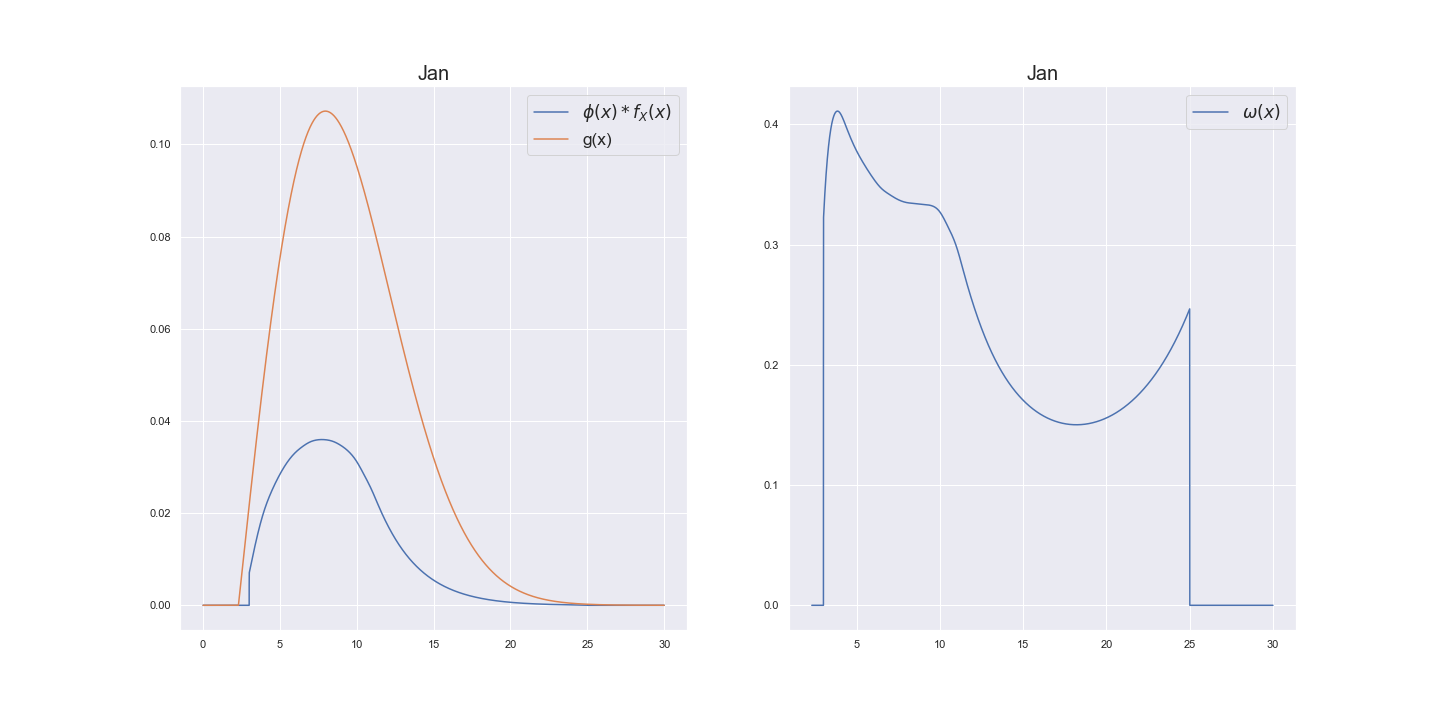
\includegraphics[width = 1.0\textwidth]{images/janPowerRatio}
    \caption{$g(x)$ (scale-transformed) and $\phi(x)*f_X(x)$ (left) and $\omega(x)$ (right) for January}
    \label{fig:janPowerRatio}
\end{figure}

\begin{table}[H]
    \centering
    \caption{Average power ratio for a wind turbine for each month of the year}
    \label{tab:powercoeff}
    \begin{tabular}{lll}
\toprule
Month & $\tau$ [$\eta$] &       $I_{95\%}$ \\
\midrule
  Jan &      30.23 $\%$ &  $\pm$ 0.05 $\%$ \\
  Feb &       31.3 $\%$ &  $\pm$ 0.06 $\%$ \\
  Mar &      31.79 $\%$ &  $\pm$ 0.08 $\%$ \\
  Apr &      31.47 $\%$ &   $\pm$ 0.1 $\%$ \\
  May &      31.47 $\%$ &  $\pm$ 0.11 $\%$ \\
  Jun &      31.46 $\%$ &   $\pm$ 0.1 $\%$ \\
  Jul &      31.36 $\%$ &  $\pm$ 0.11 $\%$ \\
  Aug &      31.47 $\%$ &   $\pm$ 0.1 $\%$ \\
  Sep &      31.91 $\%$ &  $\pm$ 0.08 $\%$ \\
  Oct &      30.26 $\%$ &  $\pm$ 0.06 $\%$ \\
  Nov &      30.21 $\%$ &  $\pm$ 0.05 $\%$ \\
  Dec &       30.2 $\%$ &  $\pm$ 0.05 $\%$ \\
\bottomrule
\end{tabular}

\end{table}

\subsection*{f) Availability and Capacity factor}
We now evaluate a metric to be able to evaluate if the power production of the wind turbine is satisfactory. The two metrics to evaluate are the \textit{capacity factor}, the ratio of outout compared to the maximum possible output of $3.075MW$, as well as the \textit{availability factor}, the amount of time that the turbine is actually producing power. For the capacity factor, we divide the expected power production obtained in section 2c by the maximum power production. The availability factor is already calculated in section 2d. The yearly average of these metrics can be found in table \ref{tab:metrics}.

\begin{table}[H]
    \centering
    \caption{Yearly average of capacity factor and availability factor}
    \label{tab:metrics}
    \begin{tabular}{lrr}
\toprule
   Month &  Capacity Factor $[\%]$ &  Availability Factor $[\%]$ \\
\midrule
     Jan &                   56.32 &                       91.92 \\
     Feb &                   51.08 &                       90.75 \\
     Mar &                   47.75 &                       89.85 \\
     Apr &                   38.63 &                       85.62 \\
     May &                   37.09 &                       84.97 \\
     Jun &                   39.43 &                       85.92 \\
     Jul &                   37.11 &                       84.97 \\
     Aug &                   39.41 &                       85.92 \\
     Sep &                   47.05 &                       89.65 \\
     Oct &                   51.61 &                       89.87 \\
     Nov &                   56.30 &                       91.92 \\
     Dec &                   56.33 &                       91.92 \\
 Average &                   46.55 &                       88.61 \\
\bottomrule
\end{tabular}

\end{table}

\newpage
\section{Power production of two wind turbines}
\label{sec:twoTurbines}

\subsection*{a)}
In order to find the expectation of the sum of power production, $\mathbb{E}[P(v_1) + P(v_2)]$ we can simply find the sum of expectations, i.e $\mathbb{E}[P(v_1)] + \mathbb{E}[P(v_2)]$. Since $v_1$ and $v_2$ are identically distributed we can approximate the sum of expectations as $\mathbb{E}[P(v_1)] + \mathbb{E}[P(v_2)] = 2\mathbb{E}[P(V_1)]$, which then is reduced to a one-dimensional problem. Therefore, we use importance sampling as in section 2b) to find an estimate. Using the yearly average parameters of $\lambda = 9.13$ and $k = 1.96$ we find the estimates of the expected power production as presented in table \ref{tab:multivarRes}.

\subsection*{b)}
To find the covariance of the power production we can use the calculation
\begin{equation}
     \mathbb{C}[P(V_1), P(V_2)] = \mathbb{E}[P(V_1)P(V_2)] - \mathbb{E}[P(V_1)]\mathbb{E}[P(V_2)]
\end{equation}
Since we already know the expected power production of one wind turbine from section 3a, we now only need to find the expectation of the product of the power production. Since the power production is identically distributed for both turbines we can instead find the expectation of the squared power production. Here we will use importance sampling to find an accurate estimate. Since this problem can not be reduced to a one dimensional problem as in 3a we now need to use a two-dimensional importance sampling approach. This gives us the following functions to sample from:
\begin{equation}
    \phi(V_1, V_2) = P(V_1)P(V_2)
\end{equation}

\begin{equation}
    f_V(v_1, v_2) = f_V(v_1)f_V(v_2)[1 + \alpha(1-F_V(v_1)^p)^{q-1}(1-F_V(v_2)^p)^{q-1}(F_V(v_1)^p(1+pq)-1)(F_V(v_2)^p(1+pq)-1)]
\end{equation}

For the importance sampling distribution we set $g(v_1, v_2)$ as a bivariate normal distribution with a mean of $[12,12]$ and a covariance matrix of 
$\begin{pmatrix} 
    10 & 2 \\ 
    2 & 10 
\end{pmatrix}$. This is visualised in figure \ref{fig:mtBruno}

\begin{figure}[H]
    \centering
    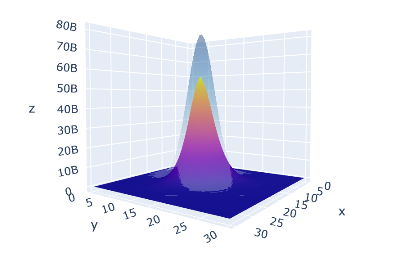
\includegraphics[width = 1.0\textwidth]{images/mtBruno}
    \caption{Importance sampling of $\mathbb{E}[P(V_1)P(V_2)]$ (opaque surface) using a bivariate normal distribution as $g(x)$ (transparent surface)}
    \label{fig:mtBruno}
\end{figure}


The results are presented in table \ref{tab:multivarRes}.

\subsection*{c)}
The variance of the combined power production can be computed using the following calculations
\begin{equation}
    \mathbb{V}[P(V_1) + P(V_2)] = \mathbb{V}[P(V_1)] + \mathbb{V}[P(V_1)] + 2\mathbb{C}[P(V_1), P(V_2)]
\end{equation}
Since we have already found all these values we simply plug them in to find the variance. The result is presented in table \ref{tab:multivarRes}.

\begin{table}[H]
    \centering
    \caption{Importance Sampling Monte Carlo estimates of the average power production of two wind turbines over a whole year}
    \label{tab:multivarRes}
    \begin{tabular}{rrrr}
\toprule
 $\mathbb{E}[P_1 + P_2] [kW]$ &  $\mathbb{C}[P_1, P_2] [kW^2]$ &  $\mathbb{V}[P_1 + P_2] [kW^2]$ &  $\mathbb{D}[P_1 + P_2] [kW] $ \\
\midrule
                      2902.66 &                   7.632802e+08 &                    4.427196e+09 &                        2104.09 \\
\bottomrule
\end{tabular}

\end{table}

\subsection*{d)}

\subsubsection*{Probability that the combined power is greater than 3.075MW}

The estimation of $\mathbb{P}(P(V_1) + P(V_2) > 3.075MV)$ is done by utilizing importance sampling with the help of an indicator function. Instead of estimating the mean, the target function $\phi(V_1, V_2)$ is selected as follows:

\begin{equation}
    \phi(V_1, V_2)=\begin{cases}
        1, & P(V_1) + P(V_2) > 3.075MW\\ 
        0, & otherwise 
    \end{cases}
\end{equation}

The sum of the power of the two turbines is only greater than zero when at least one of the winds, $V_1$ or $V_2$, is between 3 and 25. This makes the area that we want to integrate over limited in the space. 

The product of the target function and the bivariate distribution, $\phi(V_1, V_2)f(V_1, V_2)$, is plotted in figure \ref{fig:3Dprob}. We then select a distribution such that $X \in \mathcal{N}(\mu, \Sigma)$, where $\mu = [10,10]$ and $\Sigma = [[15, 2], [2, 15]]$

X was drawn from G and the samples were then calculated according to the normal procedure. The probability that the sum of two turbines is grater than 3.075MW is then equal to the mean of the samples. The mean and the confidence interval can be seen in table (SÄTT IN REF HÄR).

\begin{figure}[H]
    \centering
    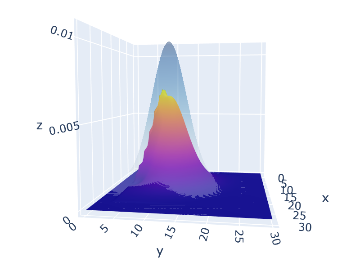
\includegraphics[width = 1.0\textwidth]{images/probability3D}
    \caption{Importance sampling of $\mathbb{P}[P(V_1) + P(V_2) > 3.075 MW]$ (Opaque surface) using a bivariate normal distribution as $g(x)$ (transparent surface)}
    \label{fig:3Dprob}
\end{figure}

\subsubsection*{Probability that the combined power is lower than 3.075MW}

To calculate the probability that the combine power is less than 3.075MW it's possible to use a similar approach as above with some modifications. We start by defining $\phi$ as:

\begin{equation}
    \phi(V_1, V_2)=\begin{cases}
        1, & P(V_1) + P(V_2) < 3.075MW\\ 
        0, & otherwise 
    \end{cases}
\end{equation}

The problem here is that the area we want to integrate over is not limited as in the task above because we now need to include all cases were the power is 0, ie either of the two wind is over 25 m/s. Because the bivariate weibull distribution is converging to zero faster than a bivariate normal distribution, we cannot select $g(x_1, x_2)$ as a multivariate normal because this will affect the variance of the estimate negatively. To solve this we did the sampling two times from a weibull distribution instead.

\end{document}
